\documentclass[11pt,twoside]{article}
\usepackage[fancy]{mdas}

\title{Trees Using Tikz}
\author{Manoj Das}

\date{\today}

\begin{document}

\maketitle
\section{Basic Tree}
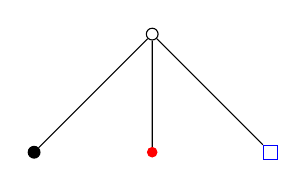
\begin{tikzpicture}
    \tikzstyle{hollow node}=[circle,draw,inner sep=1.5]
    \tikzstyle{solid node}=[circle,draw,inner sep=1.5,fill=black]
    \tikzset{
    red node/.style={circle,draw=red,fill=red,inner sep=1.2},
    blue node/.style={rectangle,draw=blue,inner sep=2.5}
    }
    \node[hollow node]{}
    child{node[solid node]{}}
    child{node[red node]{}}
    child{node[blue node]{}}
    ;
\end{tikzpicture}

\section{Game Examples}
\subsection{Tree with Circles}
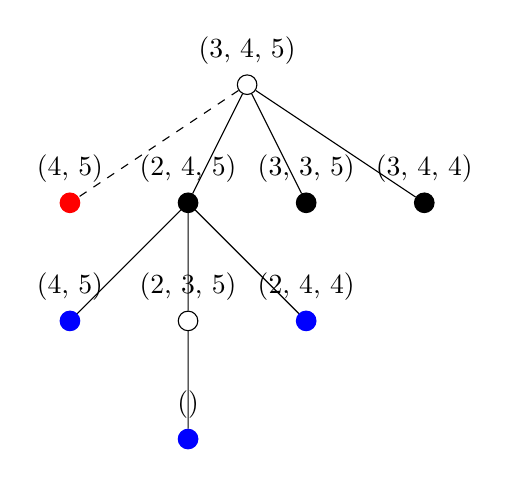
\begin{tikzpicture}
    \tikzstyle{hollow node}=[circle,draw,inner sep=2.5]
    \tikzstyle{solid node}=[circle,draw,inner sep=2.5,fill=black]
    \tikzset{
    red node/.style={circle,draw=red,fill=red,inner sep=2.5},
    blue node/.style={circle,draw=blue,fill=blue, inner sep=2.5},
    }
    \node[hollow node, label=above:{(3, 4, 5)}]{}
    child{node[red node, label=above:{(4, 5)}]{} edge from parent[dashed]}
    child{node[solid node, label=above:{(2, 4, 5)}]{} 
        child{node[blue node, label=above:{(4, 5)}]{}}
        child{node[hollow node, label=above:{(2, 3, 5)}]{} 
            child{node[blue node, label=above:{(\TBD)}]{}}
        }
        child{node[blue node, label=above:{(2, 4, 4)}]{}}
    }
    child{node[solid node, label=above:{(3, 3, 5)}]{}}
    child{node[solid node, label=above:{(3, 4, 4)}]{}}

    ;
\end{tikzpicture}

\subsection{Problem 11}
\begin{tikzpicture}
    [
    level 1/.style = {blue, sibling distance = 2.5cm},
    level 2/.style = {red, sibling distance = 4cm},
    level 3/.style = {blue, sibling distance = 2.5cm},
    level 4/.style = {red, sibling distance = 4cm},
    level 5/.style = {blue, sibling distance = 2.5cm},
    level 6/.style = {red, sibling distance = 4cm},
    level 7/.style = {blue, sibling distance = 2.5cm},
    level 8/.style = {red, sibling distance = 4cm},    
    ]
    \tikzstyle{hollow node}=[circle,draw,inner sep=2.5]
    \tikzstyle{solid node}=[circle,draw,inner sep=2.5,fill=black]
    \tikzstyle{win node}=[rectangle,draw=blue,inner sep=2.5]

    \node[]{(3,4,5,6)}
    child{node[]{(2,4,5,6)} 
        child{node[]{(4,5,6)}
            child{node[win node]{(4,4,6=6)}} 
        }
        child{node[]{(2,3,5,6)}
            child{node[]{(2,5,6)}
                child{node[]{(5,6)}
                    child{node[win node]{(5,5)}}
                }
                child{node[win node]{(2,5,5 = 2)}}
                child{node[]{(2,4,6)}
                    child{node[]{(4,6)}
                        child{node[]{(4,5)}
                            child{node[win node]{(4,4)}}
                        }
                        child{node[]{(3,6)}
                            child{node[win node]{(6)}}
                        }
                    }
                }    
            }
        } 
        child{node[]{(2,4,4,6=2,6)}
            child{node[win node]{(6)}}
        }
        child{node[]{(2,4,5,5=2,4)}
            child{node[win node]{(4)}}
        }
    }
    ;
\end{tikzpicture}

\section{References}
\begin{itemize}
    \item \url{https://latexdraw.com/draw-trees-in-tikz/}
    \item \url{https://www.sfu.ca/~haiyunc/notes/Game_Trees_with_TikZ.pdf}
\end{itemize}


\end{document}